\documentclass[10pt,twocolumn,letterpaper]{article}

\usepackage{iccv}
\usepackage{times}
\usepackage{epsfig}
\usepackage{graphicx}
\usepackage{amsmath}
\usepackage{amssymb}

% Include other packages here, before hyperref.

% If you comment hyperref and then uncomment it, you should delete
% egpaper.aux before re-running latex.  (Or just hit 'q' on the first latex
% run, let it finish, and you should be clear).

\usepackage[pagebackref=true,breaklinks=true,letterpaper=true,colorlinks,bookmarks=false]{hyperref}

\iccvfinalcopy % *** Uncomment this line for the final submission

\def\iccvPaperID{****} % *** Enter the ICCV Paper ID here
\def\httilde{\mbox{\tt\raisebox{-.5ex}{\symbol{126}}}}

% Pages are numbered in submission mode, and unnumbered in camera-ready
\ificcvfinal\pagestyle{empty}\fi

\begin{document}

  \title{Summary of Meshtalk WIP}

  \author{Jay \\
    CAU EAI Lab \\
    Lab address Here\\
    {https://yukinyaa.github.io}
  }
  \maketitle
  \thispagestyle{empty}

  \begin{abstract}
    The article summarizes Meshtalk\cite{richard2021meshtalk}.
    The goal of this practice is to get familiar with \LaTeX{} and technical writing(hopefully).
  \end{abstract}


  \section{Introduction to Meshtalk}
    Meshtalk is a generic method for generating full facial mesh animation from speech. It can generate lip-sync animation from a single frame of generic human facial mesh, and also can mix in emotional information from mesh animation.

      
    \subsection{Dataset}
      \begin{table}
        \begin{center}
          \begin{tabular}{|c||c c|}
              \hline
                Data Class & Resolution & Frame rate \\
              \hline\hline
                Face Video & 80 cameras & 30 FPS \\
                Face Mesh & 1,672 vertices & 30 FPS \\
              \hline
                Audio & 16kHz & - \\
                Mel Spectrogram & 80 Dimension & 10ms(100 FPS) \\
              \hline
          \end{tabular}
        \end{center}
        \caption{Captured, then processed Datasets}
        \label{table:dataset}
      \end{table}
      In total, there are 1.4 million frames of  13 hours equivalent audio-visual dataset from 250 subjects, reading 50 phonetically balanced sentences.

      For training dataset, first 40 sentences out of 50 \textit{about} 200 out of 250 subjects, total $40\times 200$ dataset is used for training. For evaluation, remaining 10 sentences of 50 subjects are used.
      \subsubsection*{Mesh Dataset}
      Face motion is captured with synchronized cameras, and processed into high-detail mesh, including eyelid, hairstyle, etc.
      \subsubsection*{Audio Dataset}
      Audio data is recorded in 16kHz as shown on Table \ref{table:dataset}.
      For every mesh, 600ms of audio snippet is processed info Mel spectrogram, every 10ms, in 80 dimension. Hence, \(\mathsf{a}_t \in \mathbb{R}^{60 \times 80}\)      
 
    \subsection{Network Design}


    \begin{figure}[t]
      \begin{center}
      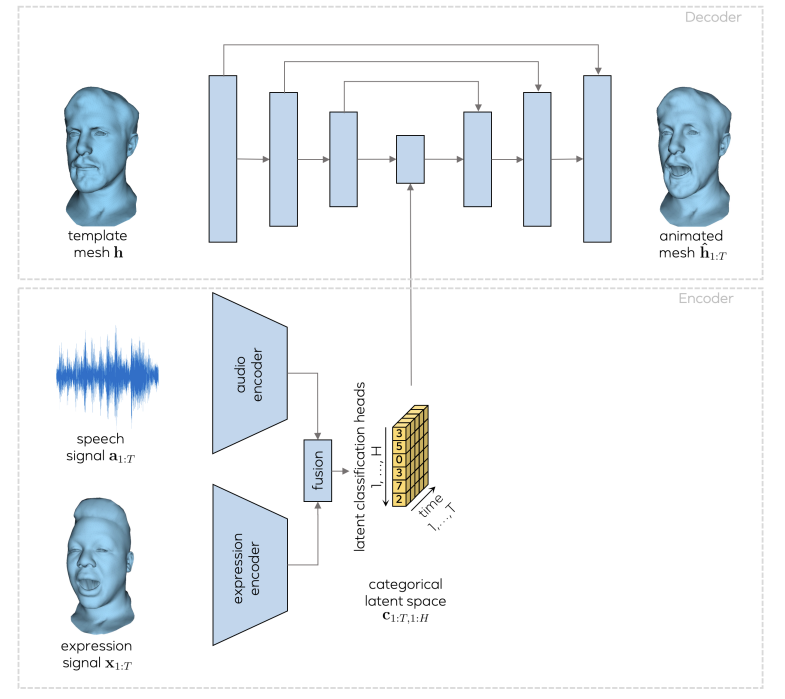
\includegraphics[width=0.8\linewidth]{meshtalk_overview.png}
      \end{center}
      \caption{The network diagram\cite{richard2021meshtalk}.}
      \label{fig:long}
      \label{fig:networkdiag}
    \end{figure}

    The network resembles Variational Autoencoder with multiple latent space as shown in Figure \ref{fig:networkdiag}.
    Target mesh \(\hat{h}\) is estimated from template mesh \(h\) and latent space \(\mathsf{c}\) by computing function \(\mathcal{D}\).
    \begin{equation}
      \hat{h}_{1:T} = \mathcal{D}(h, \mathsf{c}_{1:T, 1:H})
      \label{eq:1}
    \end{equation}
    Sequence of latent space \(\mathsf{c}_{1:T}\) is derived from audio sequence \(\mathsf{a}_{1:T}\) and expression signal mesh sequence \(\mathsf{x}_{1:T}\).
    \(c\) and \(a\) are first mapped to \(T*H*C\) dimensional latent space, then passed through Gumbel-softmax\cite{jang2017categorical} over every classification head.
    \begin{equation}
      \mathsf{c}_{1:T, 1:H} = [\mathsf{Gumbel}(\mathsf{enc}_{t,h,1:C})]_{1:T, 1:H}
    \end{equation}
    \begin{equation}
      \mathsf{enc}_{1:T,1:H,1:C} = \tilde{\xi}(x_{1:T}, a_{1:T}) 
    \end{equation}
  
    \pagebreak  
    
    \subsection{Training}
      The solution uses a novel cross-modality loss for calculating loss function for the network.
      \begin{equation}
        \begin{split}
          \mathcal{L}_{\mathsf{x}Mod} &= 
            \sum_{t=1}^{T}
            \sum_{v=1}^{V}
            \mathcal{M}_v^{\mathsf{(upper)}}
            (||\hat{h}_{t,v}^{\mathsf{(expr)}} - x_{t,v}||)\\
            &+
            \sum_{t=1}^{T}
            \sum_{v=1}^{V}
            \mathcal{M}_v^{\mathsf{(mouth)}}
            (||\hat{h}_{t,v}^{\mathsf{(audio)}} - x_{t,v}||)  
        \end{split}
      \end{equation}
      Where \(\hat{h}_{t,v}^{\mathsf{(expr)}}\) is estimated with correct expression signal and random speech signal, and
      \(\mathcal{M}^{(upper)}\) is a mask that assigned a higher weight to vertices around the mouth, and low weight to others.
      Correspondingly, \(\hat{h}_{t,v}^{\mathsf{(audio)}}\) is estimated with random expression signal and random speech signal.
      \(\mathcal{M}^{(mouth)}\) is a mask that assigns a lower weight around the mouth, and vice versa.
      Loss for eye is defined as following.
      \begin{equation}
          \mathcal{L}_{\mathsf{eyelid}} = 
            \sum_{t=1}^{T}
            \sum_{v=1}^{V}
            \mathcal{M}_v^{\mathsf{(eyelid)}}
            (||\hat{h}_{t,v}^{\mathsf{(expr)}} - x_{t,v}||)
      \end{equation}
      
      \(\mathcal{M}^{(eyelid)}\) is a specific eye loss, which was crucial.
      
      Final Loss term is defined as \(\mathcal{L} =\mathcal{L}_{\mathsf{x}Mod}+\mathcal{L}_{\mathsf{eyelid}} \), which gives both term equal weight.
  \section{Evaluation}
      To evaluate the network, the network is compared with various other networks with both numerical analysis and user-study.
    \subsection{multi-model input}
      The network is compared with  networks that lacks speech signal and uses \(\ell_2\) loss, and identical network with Meshtalk trained with \(\ell_2\) loss.
      Evaluation strategy is perplexity \(PP = p(c_{1:T,1:H}|a_{1:T})^(1\frac{1}{T*H})\) in this case.
    \subsection{Disentanglement evaluation}
      Latent space is visualized to demonstrate latent configurations that are affected by audio input and expression input are well separated to each other.
      Also, vertexes affected by each feature are computed.
      Interesting feature is that not only jaw and lip vertexes are affected by audio, but also eyebrow is significantly affected.
    \subsection{lip-vertex error}
      Lip-vertex error rate(in maximal \(\ell_2\) error, mm) is computed, and compared with VOCA\cite{Cudeiro_2019_CVPR}.
      
    \subsection{Perceptual evaluation}
    \begin{table}
      \begin{center}
        \begin{tabular}{c  c c c|c}
            \hline
               & favorability & & & ours better or equal \\
            \hline
              & competitor & equal & ours \\
            \hline
              ours vs VOCA\cite{Cudeiro_2019_CVPR} \\
              full-face & 24.7\% & 20.9\% & 54.4\% & 75.3\% \\
              lip sync & 24.7\% & 20.9\% & 54.4\% & 75.3\% \\
              upper face & 24.7\% & 20.9\% & 54.4\% & 75.3\% \\
            \hline
            ours vs ground truth \\
            full-face & 24.7\% & 20.9\% & 54.4\% & 75.3\% \\
            lip sync & 24.7\% & 20.9\% & 54.4\% & 75.3\% \\
            upper face & 24.7\% & 20.9\% & 54.4\% & 75.3\% \\
            \hline
        \end{tabular}
      \end{center}
      \caption{Perceptual study}
      \label{table:eval_favorability}
    \end{table}
      Compared with VOCA and ground truth, user study is conducted, result is shown at \ref{table:eval_favorability}
    \subsection{examples}
      Example with re-targeting, dubbing is demonstrated
    \section{limitation}
      (1) Look-ahead about 100ms is required for audio input. This is beneficial for lip-sync for sound such as '\\p'.
      (2) The model cannot be ran in real-time on low-cost devices. (3) If software fails to track certain parts, correlation fails. e.g hair overlaps eyebrow.
    
%%%%%%%%%%%%%%%%%%%%%%% References %%%%%%%%%%%%%%%%%%%%%%%%%

{
  \small
  \bibliographystyle{ieee}
  \bibliography{ref}
}

\end{document}


